\documentclass[a4paper]{book}
\usepackage{a4wide}
\usepackage{makeidx}
\usepackage{fancyhdr}
\usepackage{graphicx}
\usepackage{multicol}
\usepackage{float}
\usepackage{textcomp}
\usepackage{alltt}
\usepackage{times}
\usepackage{ifpdf}
\ifpdf
\usepackage[pdftex,
            pagebackref=true,
            colorlinks=true,
            linkcolor=blue,
            unicode
           ]{hyperref}
\else
\usepackage[ps2pdf,
            pagebackref=true,
            colorlinks=true,
            linkcolor=blue,
            unicode
           ]{hyperref}
\usepackage{pspicture}
\fi
\usepackage[utf8]{inputenc}
\usepackage{doxygen}
\makeindex
\setcounter{tocdepth}{3}
\renewcommand{\footrulewidth}{0.4pt}
\begin{document}
\begin{titlepage}
\vspace*{7cm}
\begin{center}
{\Large Reference Manual}\\
\vspace*{1cm}
{\large Generated by Doxygen 1.5.8}\\
\vspace*{0.5cm}
{\small Sat Nov 7 02:32:01 2009}\\
\end{center}
\end{titlepage}
\clearemptydoublepage
\pagenumbering{roman}
\tableofcontents
\clearemptydoublepage
\pagenumbering{arabic}
\chapter{Class Index}
\section{Class Hierarchy}
This inheritance list is sorted roughly, but not completely, alphabetically:\begin{CompactList}
\item \contentsline{section}{BaseAI::BaseAI}{\pageref{classBaseAI_1_1BaseAI}}{}
\begin{CompactList}
\item \contentsline{section}{AI::AI}{\pageref{classAI_1_1AI}}{}
\end{CompactList}
\item GameObject::GameObject\begin{CompactList}
\item \contentsline{section}{GameObject::Building}{\pageref{classGameObject_1_1Building}}{}
\item \contentsline{section}{GameObject::BuildingType}{\pageref{classGameObject_1_1BuildingType}}{}
\item \contentsline{section}{GameObject::Portal}{\pageref{classGameObject_1_1Portal}}{}
\item \contentsline{section}{GameObject::Terrain}{\pageref{classGameObject_1_1Terrain}}{}
\item \contentsline{section}{GameObject::Unit}{\pageref{classGameObject_1_1Unit}}{}
\item \contentsline{section}{GameObject::UnitType}{\pageref{classGameObject_1_1UnitType}}{}
\end{CompactList}
\end{CompactList}

\chapter{Class Index}
\section{Class List}
Here are the classes, structs, unions and interfaces with brief descriptions:\begin{CompactList}
\item\contentsline{section}{\hyperlink{classAI}{AI} (The class implementing gameplay logic )}{\pageref{classAI}}{}
\item\contentsline{section}{\hyperlink{classBaseAI}{BaseAI} (A basic \hyperlink{classAI}{AI} interface )}{\pageref{classBaseAI}}{}
\item\contentsline{section}{\hyperlink{classBuilding}{Building} (A building to shelter, feed, and/or create units )}{\pageref{classBuilding}}{}
\item\contentsline{section}{\hyperlink{classBuildingType}{BuildingType} (This defines the attributes of a kind of building )}{\pageref{classBuildingType}}{}
\item\contentsline{section}{\hyperlink{classPortal}{Portal} (A connection between two adjacent times )}{\pageref{classPortal}}{}
\item\contentsline{section}{\hyperlink{classTerrain}{Terrain} (The attributes of a specific tile of the world )}{\pageref{classTerrain}}{}
\item\contentsline{section}{\hyperlink{classUnit}{Unit} (An entitiy that can move around the game and act )}{\pageref{classUnit}}{}
\item\contentsline{section}{\hyperlink{classUnitType}{UnitType} (This defines the attributes of a kind of unit )}{\pageref{classUnitType}}{}
\end{CompactList}

\chapter{Class Documentation}
\hypertarget{classAI_1_1AI}{
\section{AI::AI Class Reference}
\label{classAI_1_1AI}\index{AI::AI@{AI::AI}}
}
Inheritance diagram for AI::AI::\begin{figure}[H]
\begin{center}
\leavevmode
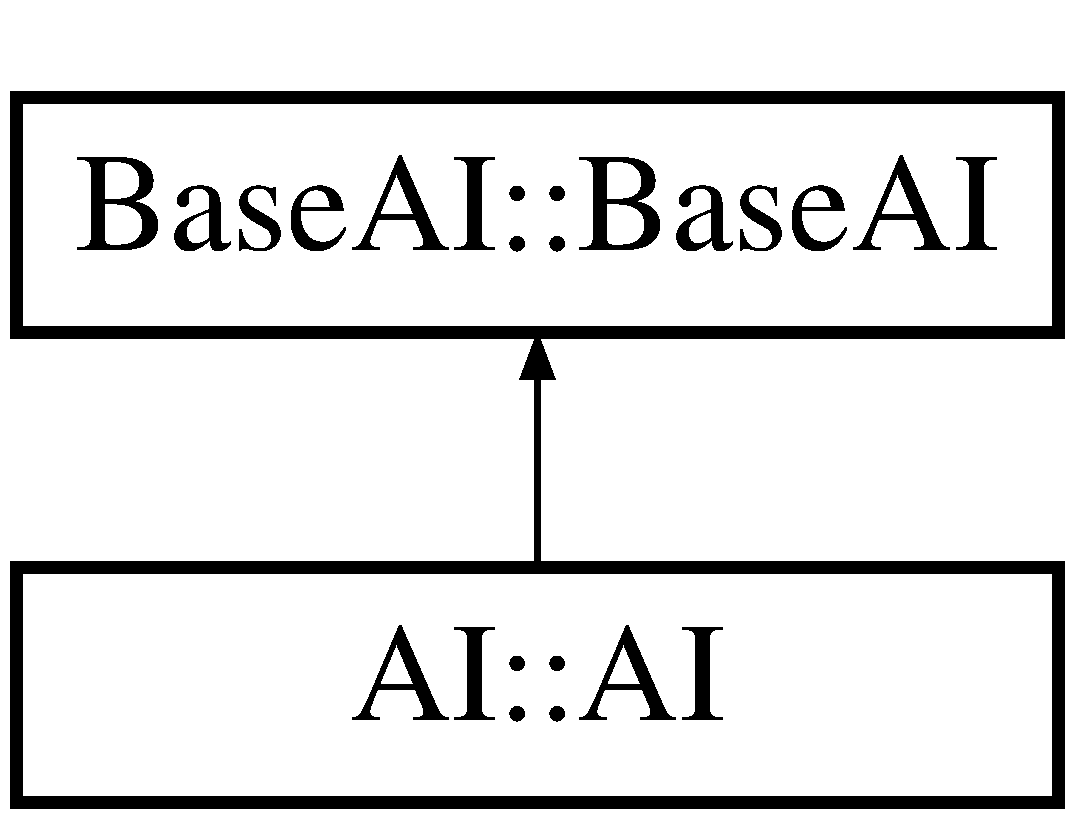
\includegraphics[height=2cm]{classAI_1_1AI}
\end{center}
\end{figure}
\subsection*{Public Member Functions}
\begin{CompactItemize}
\item 
\hypertarget{classAI_1_1AI_1173d35565e571260327628b5fdbf601}{
def \textbf{username}}
\label{classAI_1_1AI_1173d35565e571260327628b5fdbf601}

\item 
\hypertarget{classAI_1_1AI_0c68d55972c20f5b5c12b3413dccf4f8}{
def \textbf{password}}
\label{classAI_1_1AI_0c68d55972c20f5b5c12b3413dccf4f8}

\item 
\hypertarget{classAI_1_1AI_be85fa052f61e71327d0f066866360ec}{
def \textbf{init}}
\label{classAI_1_1AI_be85fa052f61e71327d0f066866360ec}

\item 
\hypertarget{classAI_1_1AI_0e95ce8db48896cbf1dcf410930ca141}{
def \textbf{run}}
\label{classAI_1_1AI_0e95ce8db48896cbf1dcf410930ca141}

\end{CompactItemize}


\subsection{Detailed Description}


\footnotesize\begin{verbatim}The class implementing gameplay logic.\end{verbatim}
\normalsize
 

The documentation for this class was generated from the following file:\begin{CompactItemize}
\item 
AI.py\end{CompactItemize}

\hypertarget{classBaseAI_1_1BaseAI}{
\section{BaseAI::BaseAI Class Reference}
\label{classBaseAI_1_1BaseAI}\index{BaseAI::BaseAI@{BaseAI::BaseAI}}
}
Inheritance diagram for BaseAI::BaseAI::\begin{figure}[H]
\begin{center}
\leavevmode
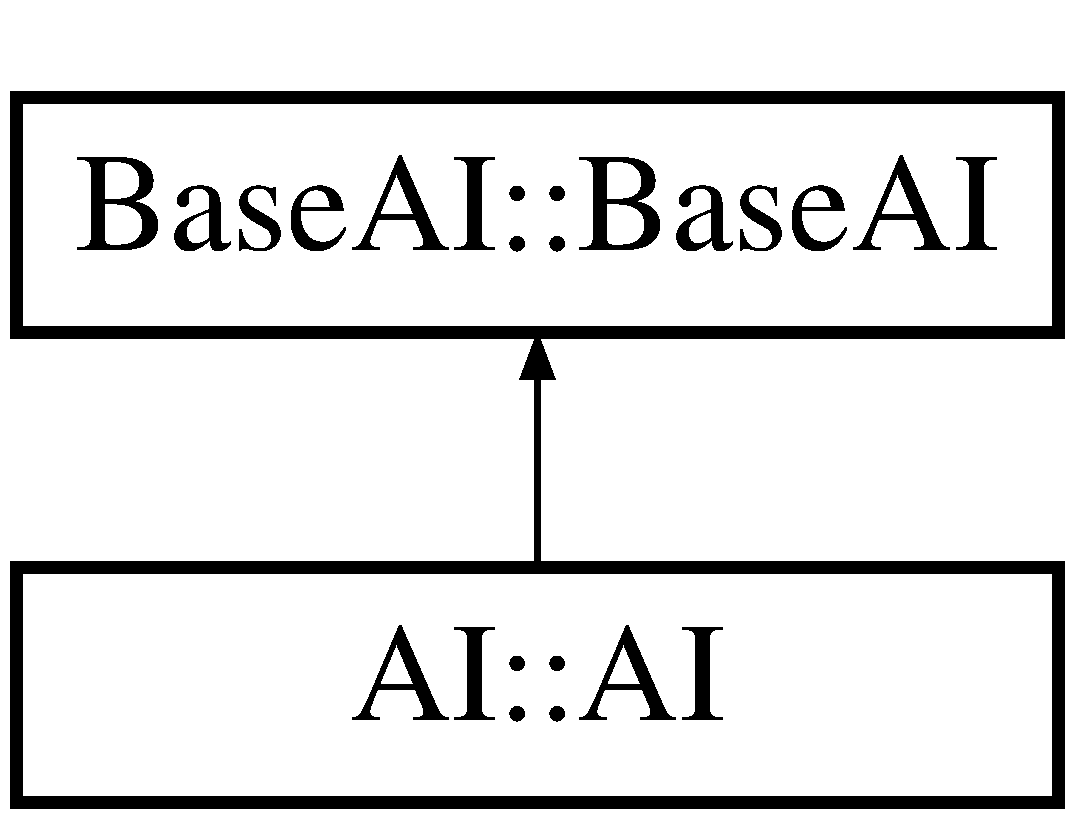
\includegraphics[height=2cm]{classBaseAI_1_1BaseAI}
\end{center}
\end{figure}
\subsection*{Public Member Functions}
\begin{CompactItemize}
\item 
\hypertarget{classBaseAI_1_1BaseAI_2dcbc8732112a39869c75ed9f0771633}{
def \textbf{startTurn}}
\label{classBaseAI_1_1BaseAI_2dcbc8732112a39869c75ed9f0771633}

\item 
\hypertarget{classBaseAI_1_1BaseAI_2af064bcf3d6dc39cc12e6817b7250b0}{
def \textbf{maxX}}
\label{classBaseAI_1_1BaseAI_2af064bcf3d6dc39cc12e6817b7250b0}

\item 
\hypertarget{classBaseAI_1_1BaseAI_80d4e182743f2508af412b9bc6a8199c}{
def \textbf{maxY}}
\label{classBaseAI_1_1BaseAI_80d4e182743f2508af412b9bc6a8199c}

\item 
def \hyperlink{classBaseAI_1_1BaseAI_65c8f75088ac56f1eca6021bf4354059}{player0Gold0}
\item 
def \hyperlink{classBaseAI_1_1BaseAI_a94399280c90f9b944a3f8c53f46d187}{player0Gold1}
\item 
def \hyperlink{classBaseAI_1_1BaseAI_bc66afa5fd654c32639a40a4574d245e}{player0Gold2}
\item 
def \hyperlink{classBaseAI_1_1BaseAI_011f11f02555a0df44af4de27b0647b0}{player1Gold0}
\item 
def \hyperlink{classBaseAI_1_1BaseAI_e1ed9b73e407052b12422e1fbea89ff0}{player1Gold1}
\item 
def \hyperlink{classBaseAI_1_1BaseAI_f9137f6d3da694e0b7af0328478d2200}{player1Gold2}
\item 
def \hyperlink{classBaseAI_1_1BaseAI_60e0d6b3832faae7c85b4c9f0be10196}{playerID}
\item 
\hypertarget{classBaseAI_1_1BaseAI_fa3d3ad590dd453c4d064a3c16b7f1a8}{
def \textbf{turnNumber}}
\label{classBaseAI_1_1BaseAI_fa3d3ad590dd453c4d064a3c16b7f1a8}

\item 
\hypertarget{classBaseAI_1_1BaseAI_7498e24706e59d7f17240c467d5b8bee}{
def \textbf{getTypeFromUnit}}
\label{classBaseAI_1_1BaseAI_7498e24706e59d7f17240c467d5b8bee}

\item 
\hypertarget{classBaseAI_1_1BaseAI_25b93552cbb6c036c0a6e2071132f3ee}{
def \textbf{getTypeFromBuilding}}
\label{classBaseAI_1_1BaseAI_25b93552cbb6c036c0a6e2071132f3ee}

\item 
def \hyperlink{classBaseAI_1_1BaseAI_95c13bf29ef95817a34f9864906e6d7c}{canMove}
\item 
def \hyperlink{classBaseAI_1_1BaseAI_e8e45448fc6bab4381fa3dd13cde748d}{canBuild}
\item 
def \hyperlink{classBaseAI_1_1BaseAI_a65ecba249b1a0b5e57e1239743a78a1}{effDamage}
\item 
def \hyperlink{classBaseAI_1_1BaseAI_3be07e2721397adc75bb376159e0bae2}{effFood}
\item 
def \hyperlink{classBaseAI_1_1BaseAI_6d1450fe6668e21e1a9e76fb4ed091b4}{getGold}
\item 
def \hyperlink{classBaseAI_1_1BaseAI_96f7fbd41f9da73ab203bc66bfabf290}{artWorth}
\item 
def \hyperlink{classBaseAI_1_1BaseAI_38e07336c6f26c483da30f2098537e1a}{hunger}
\item 
def \hyperlink{classBaseAI_1_1BaseAI_ac24297bd8420f5a88fea0f3d37bef0d}{foodProduced}
\item 
def \hyperlink{classBaseAI_1_1BaseAI_da46b6cfd17f40ab4486661143cf8429}{effBuildingPrice}
\item 
def \hyperlink{classBaseAI_1_1BaseAI_2c1cbac9339eaa991103a57645e15988}{effUnitPrice}
\item 
def \hyperlink{classBaseAI_1_1BaseAI_3ee6663a189eabaa5755c2f2f205c7fd}{effUnitMaxHP}
\item 
def \hyperlink{classBaseAI_1_1BaseAI_cc15a4773a869b4d07cca9f153e4bd03}{effBuildingMaxHP}
\item 
def \hyperlink{classBaseAI_1_1BaseAI_634977ac1854b93727b2bd6298ad2f56}{effBuildingArmor}
\item 
def \hyperlink{classBaseAI_1_1BaseAI_1dd31cd1b03afcc70ce557189d9ee1b5}{effUnitArmor}
\end{CompactItemize}
\subsection*{Static Public Attributes}
\begin{CompactItemize}
\item 
\hypertarget{classBaseAI_1_1BaseAI_32a836eb9aad27c111583f24238a686c}{
\textbf{initialized} = False}
\label{classBaseAI_1_1BaseAI_32a836eb9aad27c111583f24238a686c}

\item 
\hypertarget{classBaseAI_1_1BaseAI_54d7182ce68d3d2b55d247c431561f9d}{
int \textbf{iteration} = 0}
\label{classBaseAI_1_1BaseAI_54d7182ce68d3d2b55d247c431561f9d}

\item 
\hypertarget{classBaseAI_1_1BaseAI_e6e3fc5e4bda0d17a3ebe47365ef9e09}{
list \textbf{buildings} = \mbox{[}$\,$\mbox{]}}
\label{classBaseAI_1_1BaseAI_e6e3fc5e4bda0d17a3ebe47365ef9e09}

\item 
\hypertarget{classBaseAI_1_1BaseAI_14e8f0808f6288a31586468df99e1234}{
list \textbf{buildingTypes} = \mbox{[}$\,$\mbox{]}}
\label{classBaseAI_1_1BaseAI_14e8f0808f6288a31586468df99e1234}

\item 
\hypertarget{classBaseAI_1_1BaseAI_000a49539295be5f1fa7b7bc309989b5}{
list \textbf{portals} = \mbox{[}$\,$\mbox{]}}
\label{classBaseAI_1_1BaseAI_000a49539295be5f1fa7b7bc309989b5}

\item 
\hypertarget{classBaseAI_1_1BaseAI_945bab98670b912c7dd7cbfd498f4b69}{
list \textbf{terrains} = \mbox{[}$\,$\mbox{]}}
\label{classBaseAI_1_1BaseAI_945bab98670b912c7dd7cbfd498f4b69}

\item 
\hypertarget{classBaseAI_1_1BaseAI_4a3737dc78fb1ccb32781a1b04aa9ff6}{
list \textbf{units} = \mbox{[}$\,$\mbox{]}}
\label{classBaseAI_1_1BaseAI_4a3737dc78fb1ccb32781a1b04aa9ff6}

\item 
\hypertarget{classBaseAI_1_1BaseAI_405267241d7a9f7545b88b89a8d07ab8}{
list \textbf{unitTypes} = \mbox{[}$\,$\mbox{]}}
\label{classBaseAI_1_1BaseAI_405267241d7a9f7545b88b89a8d07ab8}

\end{CompactItemize}


\subsection{Detailed Description}


\footnotesize\begin{verbatim}@brief A basic AI interface.

This class implements most the code an AI would need to interface with the lower-level game code.
AIs should extend this class to get a lot of builer-plate code out of the way
The provided AI class does just that.
\end{verbatim}
\normalsize
 

\subsection{Member Function Documentation}
\hypertarget{classBaseAI_1_1BaseAI_96f7fbd41f9da73ab203bc66bfabf290}{
\index{BaseAI::BaseAI@{BaseAI::BaseAI}!artWorth@{artWorth}}
\index{artWorth@{artWorth}!BaseAI::BaseAI@{BaseAI::BaseAI}}
\subsubsection[{artWorth}]{\setlength{\rightskip}{0pt plus 5cm}def BaseAI::BaseAI::artWorth ( {\em artistLevel}, \/   {\em galleryLevel})}}
\label{classBaseAI_1_1BaseAI_96f7fbd41f9da73ab203bc66bfabf290}




\footnotesize\begin{verbatim}Amount of gold generated by artist at specified level
at gallery of specified level
\end{verbatim}
\normalsize
 \hypertarget{classBaseAI_1_1BaseAI_e8e45448fc6bab4381fa3dd13cde748d}{
\index{BaseAI::BaseAI@{BaseAI::BaseAI}!canBuild@{canBuild}}
\index{canBuild@{canBuild}!BaseAI::BaseAI@{BaseAI::BaseAI}}
\subsubsection[{canBuild}]{\setlength{\rightskip}{0pt plus 5cm}def BaseAI::BaseAI::canBuild ( {\em x}, \/   {\em y}, \/   {\em z})}}
\label{classBaseAI_1_1BaseAI_e8e45448fc6bab4381fa3dd13cde748d}




\footnotesize\begin{verbatim}Returns true if building on the square is possible
\end{verbatim}
\normalsize
 \hypertarget{classBaseAI_1_1BaseAI_95c13bf29ef95817a34f9864906e6d7c}{
\index{BaseAI::BaseAI@{BaseAI::BaseAI}!canMove@{canMove}}
\index{canMove@{canMove}!BaseAI::BaseAI@{BaseAI::BaseAI}}
\subsubsection[{canMove}]{\setlength{\rightskip}{0pt plus 5cm}def BaseAI::BaseAI::canMove ( {\em x}, \/   {\em y}, \/   {\em z})}}
\label{classBaseAI_1_1BaseAI_95c13bf29ef95817a34f9864906e6d7c}




\footnotesize\begin{verbatim}Returns true if movement to the square is possible
\end{verbatim}
\normalsize
 \hypertarget{classBaseAI_1_1BaseAI_634977ac1854b93727b2bd6298ad2f56}{
\index{BaseAI::BaseAI@{BaseAI::BaseAI}!effBuildingArmor@{effBuildingArmor}}
\index{effBuildingArmor@{effBuildingArmor}!BaseAI::BaseAI@{BaseAI::BaseAI}}
\subsubsection[{effBuildingArmor}]{\setlength{\rightskip}{0pt plus 5cm}def BaseAI::BaseAI::effBuildingArmor ( {\em buildingType}, \/   {\em level})}}
\label{classBaseAI_1_1BaseAI_634977ac1854b93727b2bd6298ad2f56}




\footnotesize\begin{verbatim}Armor value of building at specified level
\end{verbatim}
\normalsize
 \hypertarget{classBaseAI_1_1BaseAI_cc15a4773a869b4d07cca9f153e4bd03}{
\index{BaseAI::BaseAI@{BaseAI::BaseAI}!effBuildingMaxHP@{effBuildingMaxHP}}
\index{effBuildingMaxHP@{effBuildingMaxHP}!BaseAI::BaseAI@{BaseAI::BaseAI}}
\subsubsection[{effBuildingMaxHP}]{\setlength{\rightskip}{0pt plus 5cm}def BaseAI::BaseAI::effBuildingMaxHP ( {\em buildingType}, \/   {\em level})}}
\label{classBaseAI_1_1BaseAI_cc15a4773a869b4d07cca9f153e4bd03}




\footnotesize\begin{verbatim}Effective max HP of unit at specified level
\end{verbatim}
\normalsize
 \hypertarget{classBaseAI_1_1BaseAI_da46b6cfd17f40ab4486661143cf8429}{
\index{BaseAI::BaseAI@{BaseAI::BaseAI}!effBuildingPrice@{effBuildingPrice}}
\index{effBuildingPrice@{effBuildingPrice}!BaseAI::BaseAI@{BaseAI::BaseAI}}
\subsubsection[{effBuildingPrice}]{\setlength{\rightskip}{0pt plus 5cm}def BaseAI::BaseAI::effBuildingPrice ( {\em buildingType}, \/   {\em level})}}
\label{classBaseAI_1_1BaseAI_da46b6cfd17f40ab4486661143cf8429}




\footnotesize\begin{verbatim}Effective price of building at specified level
\end{verbatim}
\normalsize
 \hypertarget{classBaseAI_1_1BaseAI_a65ecba249b1a0b5e57e1239743a78a1}{
\index{BaseAI::BaseAI@{BaseAI::BaseAI}!effDamage@{effDamage}}
\index{effDamage@{effDamage}!BaseAI::BaseAI@{BaseAI::BaseAI}}
\subsubsection[{effDamage}]{\setlength{\rightskip}{0pt plus 5cm}def BaseAI::BaseAI::effDamage ( {\em unitType}, \/   {\em level})}}
\label{classBaseAI_1_1BaseAI_a65ecba249b1a0b5e57e1239743a78a1}




\footnotesize\begin{verbatim}Attack damage of unitType at level
\end{verbatim}
\normalsize
 \hypertarget{classBaseAI_1_1BaseAI_3be07e2721397adc75bb376159e0bae2}{
\index{BaseAI::BaseAI@{BaseAI::BaseAI}!effFood@{effFood}}
\index{effFood@{effFood}!BaseAI::BaseAI@{BaseAI::BaseAI}}
\subsubsection[{effFood}]{\setlength{\rightskip}{0pt plus 5cm}def BaseAI::BaseAI::effFood ( {\em buildingType}, \/   {\em level})}}
\label{classBaseAI_1_1BaseAI_3be07e2721397adc75bb376159e0bae2}




\footnotesize\begin{verbatim}Food produced by building at specified level
\end{verbatim}
\normalsize
 \hypertarget{classBaseAI_1_1BaseAI_1dd31cd1b03afcc70ce557189d9ee1b5}{
\index{BaseAI::BaseAI@{BaseAI::BaseAI}!effUnitArmor@{effUnitArmor}}
\index{effUnitArmor@{effUnitArmor}!BaseAI::BaseAI@{BaseAI::BaseAI}}
\subsubsection[{effUnitArmor}]{\setlength{\rightskip}{0pt plus 5cm}def BaseAI::BaseAI::effUnitArmor ( {\em unitType}, \/   {\em level})}}
\label{classBaseAI_1_1BaseAI_1dd31cd1b03afcc70ce557189d9ee1b5}




\footnotesize\begin{verbatim}Armor value of unit at specified level
\end{verbatim}
\normalsize
 \hypertarget{classBaseAI_1_1BaseAI_3ee6663a189eabaa5755c2f2f205c7fd}{
\index{BaseAI::BaseAI@{BaseAI::BaseAI}!effUnitMaxHP@{effUnitMaxHP}}
\index{effUnitMaxHP@{effUnitMaxHP}!BaseAI::BaseAI@{BaseAI::BaseAI}}
\subsubsection[{effUnitMaxHP}]{\setlength{\rightskip}{0pt plus 5cm}def BaseAI::BaseAI::effUnitMaxHP ( {\em unitType}, \/   {\em level})}}
\label{classBaseAI_1_1BaseAI_3ee6663a189eabaa5755c2f2f205c7fd}




\footnotesize\begin{verbatim}Effective max HP of unit at specified level
\end{verbatim}
\normalsize
 \hypertarget{classBaseAI_1_1BaseAI_2c1cbac9339eaa991103a57645e15988}{
\index{BaseAI::BaseAI@{BaseAI::BaseAI}!effUnitPrice@{effUnitPrice}}
\index{effUnitPrice@{effUnitPrice}!BaseAI::BaseAI@{BaseAI::BaseAI}}
\subsubsection[{effUnitPrice}]{\setlength{\rightskip}{0pt plus 5cm}def BaseAI::BaseAI::effUnitPrice ( {\em unitType}, \/   {\em level})}}
\label{classBaseAI_1_1BaseAI_2c1cbac9339eaa991103a57645e15988}




\footnotesize\begin{verbatim}Effective price of unit at specified level
\end{verbatim}
\normalsize
 \hypertarget{classBaseAI_1_1BaseAI_ac24297bd8420f5a88fea0f3d37bef0d}{
\index{BaseAI::BaseAI@{BaseAI::BaseAI}!foodProduced@{foodProduced}}
\index{foodProduced@{foodProduced}!BaseAI::BaseAI@{BaseAI::BaseAI}}
\subsubsection[{foodProduced}]{\setlength{\rightskip}{0pt plus 5cm}def BaseAI::BaseAI::foodProduced ( {\em playerID}, \/   {\em z})}}
\label{classBaseAI_1_1BaseAI_ac24297bd8420f5a88fea0f3d37bef0d}




\footnotesize\begin{verbatim}Amount of food player produces in time period z
\end{verbatim}
\normalsize
 \hypertarget{classBaseAI_1_1BaseAI_6d1450fe6668e21e1a9e76fb4ed091b4}{
\index{BaseAI::BaseAI@{BaseAI::BaseAI}!getGold@{getGold}}
\index{getGold@{getGold}!BaseAI::BaseAI@{BaseAI::BaseAI}}
\subsubsection[{getGold}]{\setlength{\rightskip}{0pt plus 5cm}def BaseAI::BaseAI::getGold ( {\em playerNum}, \/   {\em z})}}
\label{classBaseAI_1_1BaseAI_6d1450fe6668e21e1a9e76fb4ed091b4}




\footnotesize\begin{verbatim}Player's gold in specified time period
\end{verbatim}
\normalsize
 \hypertarget{classBaseAI_1_1BaseAI_38e07336c6f26c483da30f2098537e1a}{
\index{BaseAI::BaseAI@{BaseAI::BaseAI}!hunger@{hunger}}
\index{hunger@{hunger}!BaseAI::BaseAI@{BaseAI::BaseAI}}
\subsubsection[{hunger}]{\setlength{\rightskip}{0pt plus 5cm}def BaseAI::BaseAI::hunger ( {\em playerID}, \/   {\em z})}}
\label{classBaseAI_1_1BaseAI_38e07336c6f26c483da30f2098537e1a}




\footnotesize\begin{verbatim}Hunger damage to specified player in time period z
\end{verbatim}
\normalsize
 \hypertarget{classBaseAI_1_1BaseAI_65c8f75088ac56f1eca6021bf4354059}{
\index{BaseAI::BaseAI@{BaseAI::BaseAI}!player0Gold0@{player0Gold0}}
\index{player0Gold0@{player0Gold0}!BaseAI::BaseAI@{BaseAI::BaseAI}}
\subsubsection[{player0Gold0}]{\setlength{\rightskip}{0pt plus 5cm}def BaseAI::BaseAI::player0Gold0 ()}}
\label{classBaseAI_1_1BaseAI_65c8f75088ac56f1eca6021bf4354059}




\footnotesize\begin{verbatim}Player 0's past gold
\end{verbatim}
\normalsize
 \hypertarget{classBaseAI_1_1BaseAI_a94399280c90f9b944a3f8c53f46d187}{
\index{BaseAI::BaseAI@{BaseAI::BaseAI}!player0Gold1@{player0Gold1}}
\index{player0Gold1@{player0Gold1}!BaseAI::BaseAI@{BaseAI::BaseAI}}
\subsubsection[{player0Gold1}]{\setlength{\rightskip}{0pt plus 5cm}def BaseAI::BaseAI::player0Gold1 ()}}
\label{classBaseAI_1_1BaseAI_a94399280c90f9b944a3f8c53f46d187}




\footnotesize\begin{verbatim}Player 0's present gold
\end{verbatim}
\normalsize
 \hypertarget{classBaseAI_1_1BaseAI_bc66afa5fd654c32639a40a4574d245e}{
\index{BaseAI::BaseAI@{BaseAI::BaseAI}!player0Gold2@{player0Gold2}}
\index{player0Gold2@{player0Gold2}!BaseAI::BaseAI@{BaseAI::BaseAI}}
\subsubsection[{player0Gold2}]{\setlength{\rightskip}{0pt plus 5cm}def BaseAI::BaseAI::player0Gold2 ()}}
\label{classBaseAI_1_1BaseAI_bc66afa5fd654c32639a40a4574d245e}




\footnotesize\begin{verbatim}Player 0's future gold
\end{verbatim}
\normalsize
 \hypertarget{classBaseAI_1_1BaseAI_011f11f02555a0df44af4de27b0647b0}{
\index{BaseAI::BaseAI@{BaseAI::BaseAI}!player1Gold0@{player1Gold0}}
\index{player1Gold0@{player1Gold0}!BaseAI::BaseAI@{BaseAI::BaseAI}}
\subsubsection[{player1Gold0}]{\setlength{\rightskip}{0pt plus 5cm}def BaseAI::BaseAI::player1Gold0 ()}}
\label{classBaseAI_1_1BaseAI_011f11f02555a0df44af4de27b0647b0}




\footnotesize\begin{verbatim}Player 1's past gold
\end{verbatim}
\normalsize
 \hypertarget{classBaseAI_1_1BaseAI_e1ed9b73e407052b12422e1fbea89ff0}{
\index{BaseAI::BaseAI@{BaseAI::BaseAI}!player1Gold1@{player1Gold1}}
\index{player1Gold1@{player1Gold1}!BaseAI::BaseAI@{BaseAI::BaseAI}}
\subsubsection[{player1Gold1}]{\setlength{\rightskip}{0pt plus 5cm}def BaseAI::BaseAI::player1Gold1 ()}}
\label{classBaseAI_1_1BaseAI_e1ed9b73e407052b12422e1fbea89ff0}




\footnotesize\begin{verbatim}Player 1's present gold
\end{verbatim}
\normalsize
 \hypertarget{classBaseAI_1_1BaseAI_f9137f6d3da694e0b7af0328478d2200}{
\index{BaseAI::BaseAI@{BaseAI::BaseAI}!player1Gold2@{player1Gold2}}
\index{player1Gold2@{player1Gold2}!BaseAI::BaseAI@{BaseAI::BaseAI}}
\subsubsection[{player1Gold2}]{\setlength{\rightskip}{0pt plus 5cm}def BaseAI::BaseAI::player1Gold2 ()}}
\label{classBaseAI_1_1BaseAI_f9137f6d3da694e0b7af0328478d2200}




\footnotesize\begin{verbatim}Player 1's future gold
\end{verbatim}
\normalsize
 \hypertarget{classBaseAI_1_1BaseAI_60e0d6b3832faae7c85b4c9f0be10196}{
\index{BaseAI::BaseAI@{BaseAI::BaseAI}!playerID@{playerID}}
\index{playerID@{playerID}!BaseAI::BaseAI@{BaseAI::BaseAI}}
\subsubsection[{playerID}]{\setlength{\rightskip}{0pt plus 5cm}def BaseAI::BaseAI::playerID ()}}
\label{classBaseAI_1_1BaseAI_60e0d6b3832faae7c85b4c9f0be10196}




\footnotesize\begin{verbatim}Player Number; either 0 or 2
\end{verbatim}
\normalsize
 

The documentation for this class was generated from the following file:\begin{CompactItemize}
\item 
BaseAI.py\end{CompactItemize}

\hypertarget{classGameObject_1_1Building}{
\section{GameObject::Building Class Reference}
\label{classGameObject_1_1Building}\index{GameObject::Building@{GameObject::Building}}
}
Inheritance diagram for GameObject::Building::\begin{figure}[H]
\begin{center}
\leavevmode
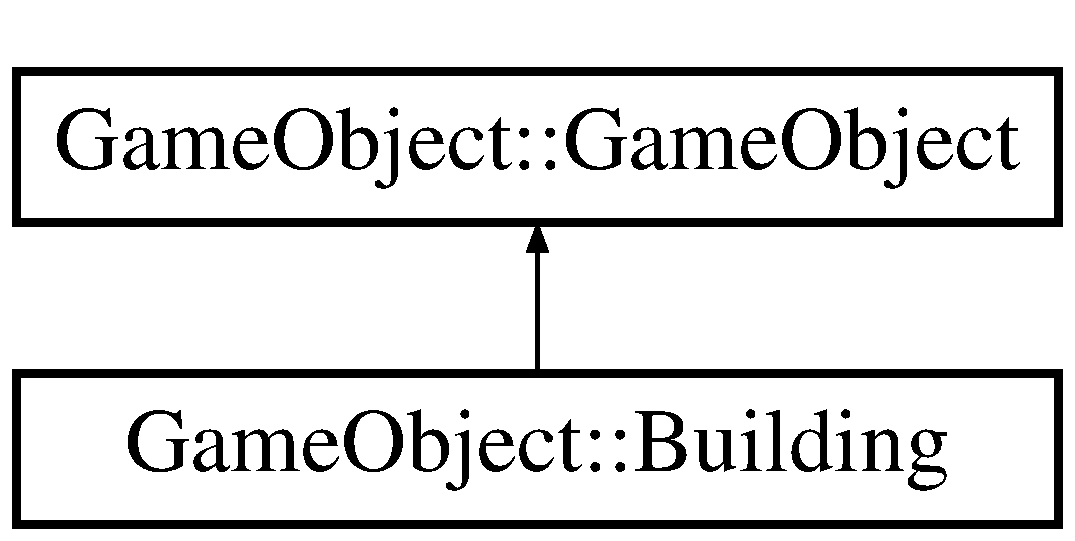
\includegraphics[height=2cm]{classGameObject_1_1Building}
\end{center}
\end{figure}
\subsection*{Public Member Functions}
\begin{CompactItemize}
\item 
\hypertarget{classGameObject_1_1Building_eb6045358dab03e17c6ba476b3a46588}{
def \textbf{\_\-\_\-init\_\-\_\-}}
\label{classGameObject_1_1Building_eb6045358dab03e17c6ba476b3a46588}

\item 
\hypertarget{classGameObject_1_1Building_daeb682b33b8a34e1bc5957c712e73b4}{
def \textbf{validify}}
\label{classGameObject_1_1Building_daeb682b33b8a34e1bc5957c712e73b4}

\item 
\hypertarget{classGameObject_1_1Building_14f30b920edbeac55eaae511820abfcd}{
def \textbf{train}}
\label{classGameObject_1_1Building_14f30b920edbeac55eaae511820abfcd}

\item 
\hypertarget{classGameObject_1_1Building_81ec3da0991b30fc87e153d71cc0b3d5}{
def \textbf{cancel}}
\label{classGameObject_1_1Building_81ec3da0991b30fc87e153d71cc0b3d5}

\item 
\hypertarget{classGameObject_1_1Building_659d12a77cc1ac007f5fe185ec51533a}{
def \textbf{getObjectID}}
\label{classGameObject_1_1Building_659d12a77cc1ac007f5fe185ec51533a}

\item 
\hypertarget{classGameObject_1_1Building_2a15365dc0fb769174320a9b23a67ed8}{
def \textbf{getX}}
\label{classGameObject_1_1Building_2a15365dc0fb769174320a9b23a67ed8}

\item 
\hypertarget{classGameObject_1_1Building_c10cc24e6b78b64cffde90eff531334d}{
def \textbf{getY}}
\label{classGameObject_1_1Building_c10cc24e6b78b64cffde90eff531334d}

\item 
\hypertarget{classGameObject_1_1Building_a4296ec82731efae607649fa52ab7319}{
def \textbf{getZ}}
\label{classGameObject_1_1Building_a4296ec82731efae607649fa52ab7319}

\item 
\hypertarget{classGameObject_1_1Building_e9dffb5ac8c59acc6beb85f82826befc}{
def \textbf{getHp}}
\label{classGameObject_1_1Building_e9dffb5ac8c59acc6beb85f82826befc}

\item 
\hypertarget{classGameObject_1_1Building_aa320a6996c96f11a159181f140b9d93}{
def \textbf{getLevel}}
\label{classGameObject_1_1Building_aa320a6996c96f11a159181f140b9d93}

\item 
\hypertarget{classGameObject_1_1Building_54a606aff2e25347bc86dd6be922243d}{
def \textbf{getBuildingTypeID}}
\label{classGameObject_1_1Building_54a606aff2e25347bc86dd6be922243d}

\item 
\hypertarget{classGameObject_1_1Building_38b3022fc69b136f6919a303e6ebe38a}{
def \textbf{getOwnerID}}
\label{classGameObject_1_1Building_38b3022fc69b136f6919a303e6ebe38a}

\item 
\hypertarget{classGameObject_1_1Building_d16ef9f3fce2ae5ad621ba38b861e8eb}{
def \textbf{getInTraining}}
\label{classGameObject_1_1Building_d16ef9f3fce2ae5ad621ba38b861e8eb}

\item 
\hypertarget{classGameObject_1_1Building_17c60f336f9ec57370a9aa66a2ce513f}{
def \textbf{getProgress}}
\label{classGameObject_1_1Building_17c60f336f9ec57370a9aa66a2ce513f}

\item 
\hypertarget{classGameObject_1_1Building_768d8e4b043a44a7a8716053a032d9c4}{
def \textbf{getLinked}}
\label{classGameObject_1_1Building_768d8e4b043a44a7a8716053a032d9c4}

\item 
\hypertarget{classGameObject_1_1Building_f65e3f7d76af3b4f59049ea28c55c5c3}{
def \textbf{getComplete}}
\label{classGameObject_1_1Building_f65e3f7d76af3b4f59049ea28c55c5c3}

\end{CompactItemize}
\subsection*{Public Attributes}
\begin{CompactItemize}
\item 
\hypertarget{classGameObject_1_1Building_75182603210be4e2339843163b9c50a1}{
\textbf{ptr}}
\label{classGameObject_1_1Building_75182603210be4e2339843163b9c50a1}

\item 
\hypertarget{classGameObject_1_1Building_72b0c8b116aacbcc5c86bbff21ffb3c0}{
\textbf{iteration}}
\label{classGameObject_1_1Building_72b0c8b116aacbcc5c86bbff21ffb3c0}

\item 
\hypertarget{classGameObject_1_1Building_408aaa29bf5784b179852119ef2cccef}{
\textbf{ID}}
\label{classGameObject_1_1Building_408aaa29bf5784b179852119ef2cccef}

\end{CompactItemize}


\subsection{Detailed Description}


\footnotesize\begin{verbatim}A building to shelter, feed, and/or create units.
\end{verbatim}
\normalsize
 

The documentation for this class was generated from the following file:\begin{CompactItemize}
\item 
GameObject.py\end{CompactItemize}

\hypertarget{classGameObject_1_1BuildingType}{
\section{GameObject::BuildingType Class Reference}
\label{classGameObject_1_1BuildingType}\index{GameObject::BuildingType@{GameObject::BuildingType}}
}
Inheritance diagram for GameObject::BuildingType::\begin{figure}[H]
\begin{center}
\leavevmode
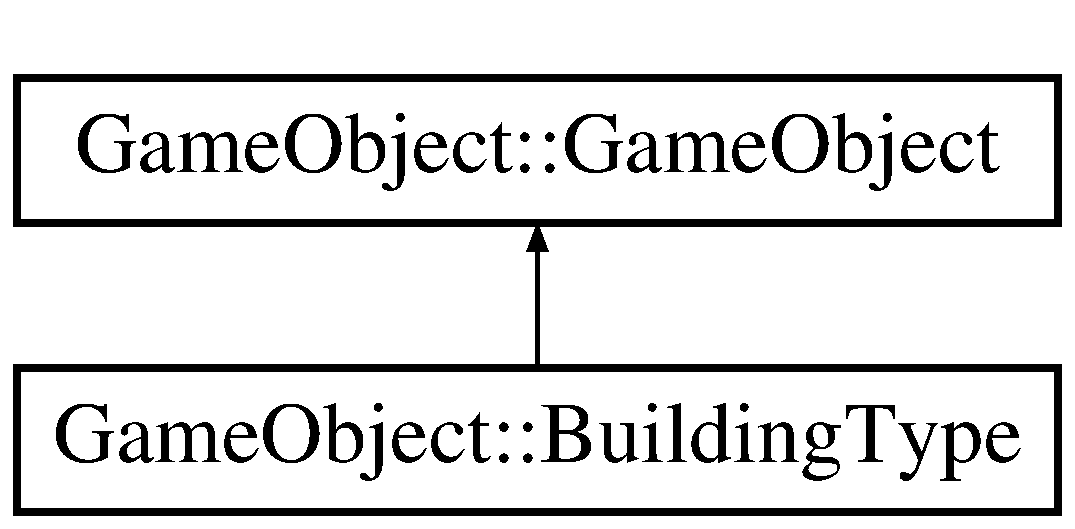
\includegraphics[height=2cm]{classGameObject_1_1BuildingType}
\end{center}
\end{figure}
\subsection*{Public Member Functions}
\begin{CompactItemize}
\item 
\hypertarget{classGameObject_1_1BuildingType_500a56f4566cefd07be88e914817ccbb}{
def \textbf{\_\-\_\-init\_\-\_\-}}
\label{classGameObject_1_1BuildingType_500a56f4566cefd07be88e914817ccbb}

\item 
\hypertarget{classGameObject_1_1BuildingType_f172800dda38b221d18f25a4dc1bbaf2}{
def \textbf{validify}}
\label{classGameObject_1_1BuildingType_f172800dda38b221d18f25a4dc1bbaf2}

\item 
\hypertarget{classGameObject_1_1BuildingType_11c5eb131d0f3f447e6c0f68978d8b08}{
def \textbf{getObjectID}}
\label{classGameObject_1_1BuildingType_11c5eb131d0f3f447e6c0f68978d8b08}

\item 
\hypertarget{classGameObject_1_1BuildingType_a07462a9e55227486613a822582326f7}{
def \textbf{getName}}
\label{classGameObject_1_1BuildingType_a07462a9e55227486613a822582326f7}

\item 
\hypertarget{classGameObject_1_1BuildingType_5d012aa14cbf81b77c48c2856b617b95}{
def \textbf{getPrice}}
\label{classGameObject_1_1BuildingType_5d012aa14cbf81b77c48c2856b617b95}

\item 
\hypertarget{classGameObject_1_1BuildingType_d6161ac34a655b9e027cbcf53e2d8477}{
def \textbf{getFood}}
\label{classGameObject_1_1BuildingType_d6161ac34a655b9e027cbcf53e2d8477}

\item 
\hypertarget{classGameObject_1_1BuildingType_51eefc9f6d5ea5f3ec39613d349c5139}{
def \textbf{getPastBuildTime}}
\label{classGameObject_1_1BuildingType_51eefc9f6d5ea5f3ec39613d349c5139}

\item 
\hypertarget{classGameObject_1_1BuildingType_7766d7ab40b1042155e2e94a54e61349}{
def \textbf{getPresentBuildTime}}
\label{classGameObject_1_1BuildingType_7766d7ab40b1042155e2e94a54e61349}

\item 
\hypertarget{classGameObject_1_1BuildingType_a37c8617bdafd18d84e051d1694c410a}{
def \textbf{getFutureBuildTime}}
\label{classGameObject_1_1BuildingType_a37c8617bdafd18d84e051d1694c410a}

\item 
\hypertarget{classGameObject_1_1BuildingType_8dd73d6e912ed516ffdb0ff6cc5b412a}{
def \textbf{getHp}}
\label{classGameObject_1_1BuildingType_8dd73d6e912ed516ffdb0ff6cc5b412a}

\item 
\hypertarget{classGameObject_1_1BuildingType_da1025962c33495c2b9d3d28839ef2d8}{
def \textbf{getArmor}}
\label{classGameObject_1_1BuildingType_da1025962c33495c2b9d3d28839ef2d8}

\item 
\hypertarget{classGameObject_1_1BuildingType_421cdb63e77b2cdfb0631bf0717a17a0}{
def \textbf{getBuilderID}}
\label{classGameObject_1_1BuildingType_421cdb63e77b2cdfb0631bf0717a17a0}

\item 
\hypertarget{classGameObject_1_1BuildingType_a5fda9f5d6812196fe2836ee9adb5d74}{
def \textbf{getAllowPaint}}
\label{classGameObject_1_1BuildingType_a5fda9f5d6812196fe2836ee9adb5d74}

\item 
\hypertarget{classGameObject_1_1BuildingType_4e65a9f1061395ac2beb578244ab8f6a}{
def \textbf{getWidth}}
\label{classGameObject_1_1BuildingType_4e65a9f1061395ac2beb578244ab8f6a}

\item 
\hypertarget{classGameObject_1_1BuildingType_a602cf5d181827c411269f19e76e7e64}{
def \textbf{getHeight}}
\label{classGameObject_1_1BuildingType_a602cf5d181827c411269f19e76e7e64}

\item 
\hypertarget{classGameObject_1_1BuildingType_100d07a3daa6c995105f534a3dc66491}{
def \textbf{getSpawnX}}
\label{classGameObject_1_1BuildingType_100d07a3daa6c995105f534a3dc66491}

\item 
\hypertarget{classGameObject_1_1BuildingType_431e74b93193361cb8eabfabec62cc10}{
def \textbf{getSpawnY}}
\label{classGameObject_1_1BuildingType_431e74b93193361cb8eabfabec62cc10}

\item 
\hypertarget{classGameObject_1_1BuildingType_4e677d90b401870eb3277b784524b943}{
def \textbf{getArmorExp}}
\label{classGameObject_1_1BuildingType_4e677d90b401870eb3277b784524b943}

\item 
\hypertarget{classGameObject_1_1BuildingType_9d522b960946cefc507f6d62976deae8}{
def \textbf{getHpExp}}
\label{classGameObject_1_1BuildingType_9d522b960946cefc507f6d62976deae8}

\item 
\hypertarget{classGameObject_1_1BuildingType_1eedfdaf909a02aa607767709d293c91}{
def \textbf{getPriceExp}}
\label{classGameObject_1_1BuildingType_1eedfdaf909a02aa607767709d293c91}

\item 
\hypertarget{classGameObject_1_1BuildingType_1adf563916b28cf075b9f6ae151685f7}{
def \textbf{getFoodExp}}
\label{classGameObject_1_1BuildingType_1adf563916b28cf075b9f6ae151685f7}

\end{CompactItemize}
\subsection*{Public Attributes}
\begin{CompactItemize}
\item 
\hypertarget{classGameObject_1_1BuildingType_24ed6d11c9c3a45f8f1ab8f5696d1e47}{
\textbf{ptr}}
\label{classGameObject_1_1BuildingType_24ed6d11c9c3a45f8f1ab8f5696d1e47}

\item 
\hypertarget{classGameObject_1_1BuildingType_6262e9784b8450dee03ed3cd8e412e3f}{
\textbf{iteration}}
\label{classGameObject_1_1BuildingType_6262e9784b8450dee03ed3cd8e412e3f}

\item 
\hypertarget{classGameObject_1_1BuildingType_12f29b224c0ab12334c94cff104ff17c}{
\textbf{ID}}
\label{classGameObject_1_1BuildingType_12f29b224c0ab12334c94cff104ff17c}

\end{CompactItemize}


\subsection{Detailed Description}


\footnotesize\begin{verbatim}This defines the attributes of a kind of building.
\end{verbatim}
\normalsize
 

The documentation for this class was generated from the following file:\begin{CompactItemize}
\item 
GameObject.py\end{CompactItemize}

\hypertarget{classGameObject_1_1Portal}{
\section{GameObject::Portal Class Reference}
\label{classGameObject_1_1Portal}\index{GameObject::Portal@{GameObject::Portal}}
}
Inheritance diagram for GameObject::Portal::\begin{figure}[H]
\begin{center}
\leavevmode
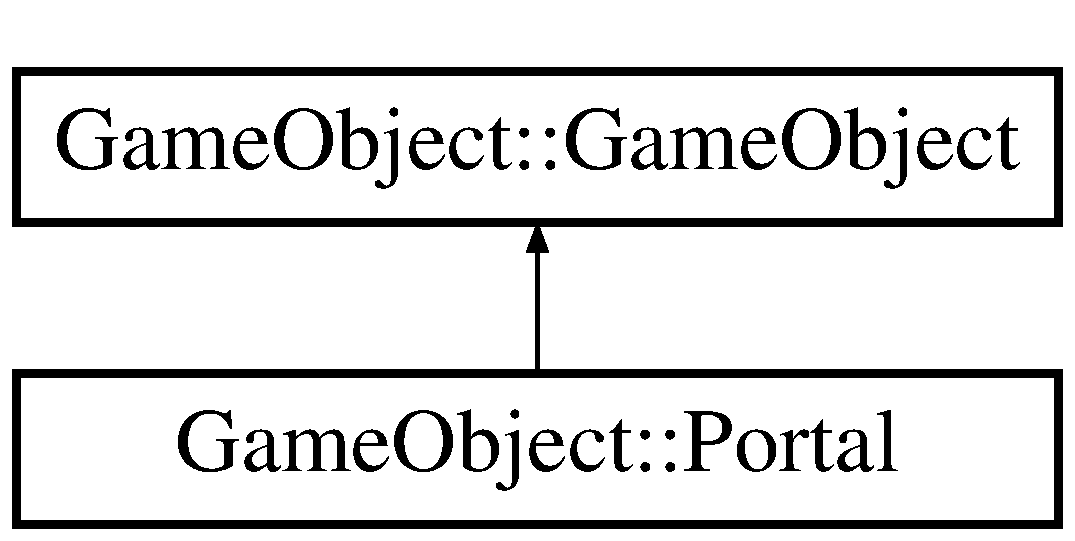
\includegraphics[height=2cm]{classGameObject_1_1Portal}
\end{center}
\end{figure}
\subsection*{Public Member Functions}
\begin{CompactItemize}
\item 
\hypertarget{classGameObject_1_1Portal_a1adc7f3fdb62ab8c27c70c1a8b3a703}{
def \textbf{\_\-\_\-init\_\-\_\-}}
\label{classGameObject_1_1Portal_a1adc7f3fdb62ab8c27c70c1a8b3a703}

\item 
\hypertarget{classGameObject_1_1Portal_46b36b978c86507377aec9dee9fc1239}{
def \textbf{validify}}
\label{classGameObject_1_1Portal_46b36b978c86507377aec9dee9fc1239}

\item 
\hypertarget{classGameObject_1_1Portal_580a57bb97d42af10459975de71fb499}{
def \textbf{getObjectID}}
\label{classGameObject_1_1Portal_580a57bb97d42af10459975de71fb499}

\item 
\hypertarget{classGameObject_1_1Portal_c359af216f892f72e8ba6ca96a6fd102}{
def \textbf{getX}}
\label{classGameObject_1_1Portal_c359af216f892f72e8ba6ca96a6fd102}

\item 
\hypertarget{classGameObject_1_1Portal_ae4cc2521dcaefc577b70085b7b810d2}{
def \textbf{getY}}
\label{classGameObject_1_1Portal_ae4cc2521dcaefc577b70085b7b810d2}

\item 
\hypertarget{classGameObject_1_1Portal_e442927b4806e1a98d690973f6ce1c30}{
def \textbf{getZ}}
\label{classGameObject_1_1Portal_e442927b4806e1a98d690973f6ce1c30}

\item 
\hypertarget{classGameObject_1_1Portal_e73b144974cf2f0a2fbb9a1122f83b99}{
def \textbf{getDirection}}
\label{classGameObject_1_1Portal_e73b144974cf2f0a2fbb9a1122f83b99}

\item 
\hypertarget{classGameObject_1_1Portal_19d3642e7f1d6575eb922316c72b51b4}{
def \textbf{getFee}}
\label{classGameObject_1_1Portal_19d3642e7f1d6575eb922316c72b51b4}

\item 
\hypertarget{classGameObject_1_1Portal_b13eb65ac9bf026d8d766359ded62572}{
def \textbf{getFeeIncr}}
\label{classGameObject_1_1Portal_b13eb65ac9bf026d8d766359ded62572}

\item 
\hypertarget{classGameObject_1_1Portal_d492840ebf3cea7299010d2dbe051c4a}{
def \textbf{getFeeMultiplier}}
\label{classGameObject_1_1Portal_d492840ebf3cea7299010d2dbe051c4a}

\end{CompactItemize}
\subsection*{Public Attributes}
\begin{CompactItemize}
\item 
\hypertarget{classGameObject_1_1Portal_b8d30df65bff59aa2336d8a1f8a266d7}{
\textbf{ptr}}
\label{classGameObject_1_1Portal_b8d30df65bff59aa2336d8a1f8a266d7}

\item 
\hypertarget{classGameObject_1_1Portal_f5373bbc57189b566748d050c4eafad5}{
\textbf{iteration}}
\label{classGameObject_1_1Portal_f5373bbc57189b566748d050c4eafad5}

\item 
\hypertarget{classGameObject_1_1Portal_b3b6e17b22187150345d32dc1cde60ed}{
\textbf{ID}}
\label{classGameObject_1_1Portal_b3b6e17b22187150345d32dc1cde60ed}

\end{CompactItemize}


\subsection{Detailed Description}


\footnotesize\begin{verbatim}A connection between two adjacent times.
\end{verbatim}
\normalsize
 

The documentation for this class was generated from the following file:\begin{CompactItemize}
\item 
GameObject.py\end{CompactItemize}

\hypertarget{classGameObject_1_1Terrain}{
\section{GameObject::Terrain Class Reference}
\label{classGameObject_1_1Terrain}\index{GameObject::Terrain@{GameObject::Terrain}}
}
Inheritance diagram for GameObject::Terrain::\begin{figure}[H]
\begin{center}
\leavevmode
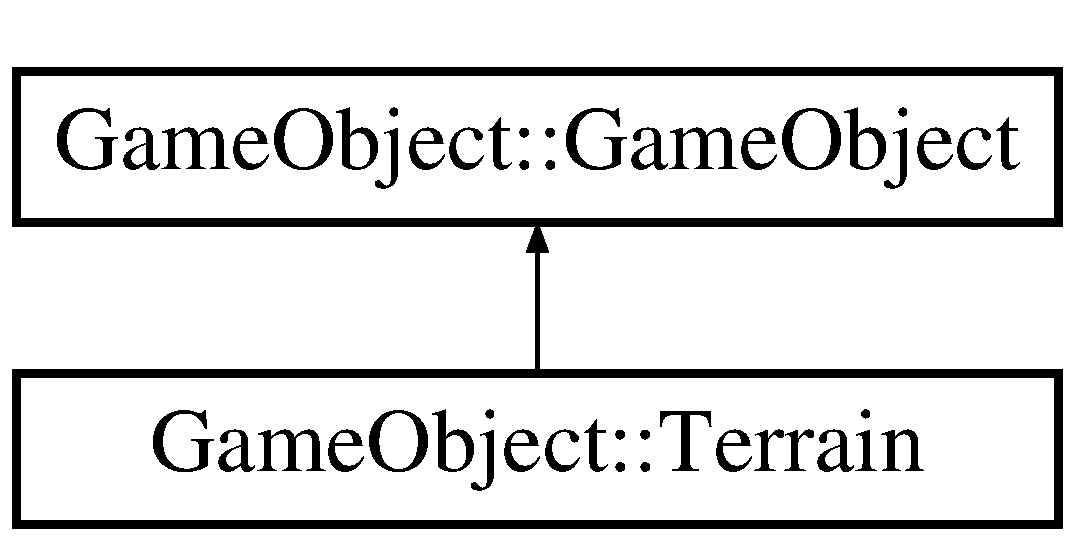
\includegraphics[height=2cm]{classGameObject_1_1Terrain}
\end{center}
\end{figure}
\subsection*{Public Member Functions}
\begin{CompactItemize}
\item 
\hypertarget{classGameObject_1_1Terrain_7cfd1b55784901ef60499589b76d5656}{
def \textbf{\_\-\_\-init\_\-\_\-}}
\label{classGameObject_1_1Terrain_7cfd1b55784901ef60499589b76d5656}

\item 
\hypertarget{classGameObject_1_1Terrain_b1195ab481b44c7f72fcfaccc600919e}{
def \textbf{validify}}
\label{classGameObject_1_1Terrain_b1195ab481b44c7f72fcfaccc600919e}

\item 
\hypertarget{classGameObject_1_1Terrain_6eecad5843e03998e089cdf06ef41d7e}{
def \textbf{getObjectID}}
\label{classGameObject_1_1Terrain_6eecad5843e03998e089cdf06ef41d7e}

\item 
\hypertarget{classGameObject_1_1Terrain_e6a5cf94fd76c215e5e2f99f3446ca03}{
def \textbf{getX}}
\label{classGameObject_1_1Terrain_e6a5cf94fd76c215e5e2f99f3446ca03}

\item 
\hypertarget{classGameObject_1_1Terrain_84913a2cf678421a5ab4a1c9202e27f6}{
def \textbf{getY}}
\label{classGameObject_1_1Terrain_84913a2cf678421a5ab4a1c9202e27f6}

\item 
\hypertarget{classGameObject_1_1Terrain_2d86f046475f501c36cfadf8098ef8fe}{
def \textbf{getZ}}
\label{classGameObject_1_1Terrain_2d86f046475f501c36cfadf8098ef8fe}

\item 
\hypertarget{classGameObject_1_1Terrain_bc5f98e0cdcf51c4fe1db124450bdc29}{
def \textbf{getBlocksMove}}
\label{classGameObject_1_1Terrain_bc5f98e0cdcf51c4fe1db124450bdc29}

\item 
\hypertarget{classGameObject_1_1Terrain_06e1d73f49fe0546fc3ab1af40998b4e}{
def \textbf{getBlocksBuild}}
\label{classGameObject_1_1Terrain_06e1d73f49fe0546fc3ab1af40998b4e}

\end{CompactItemize}
\subsection*{Public Attributes}
\begin{CompactItemize}
\item 
\hypertarget{classGameObject_1_1Terrain_074268347b24dc6cbbe328c310e7b7a1}{
\textbf{ptr}}
\label{classGameObject_1_1Terrain_074268347b24dc6cbbe328c310e7b7a1}

\item 
\hypertarget{classGameObject_1_1Terrain_204c37c466d3f8036afeb191823dc558}{
\textbf{iteration}}
\label{classGameObject_1_1Terrain_204c37c466d3f8036afeb191823dc558}

\item 
\hypertarget{classGameObject_1_1Terrain_a32339fa2347c1b9ab533d0bd94b3132}{
\textbf{ID}}
\label{classGameObject_1_1Terrain_a32339fa2347c1b9ab533d0bd94b3132}

\end{CompactItemize}


\subsection{Detailed Description}


\footnotesize\begin{verbatim}The attributes of a specific tile of the world.
\end{verbatim}
\normalsize
 

The documentation for this class was generated from the following file:\begin{CompactItemize}
\item 
GameObject.py\end{CompactItemize}

\hypertarget{classGameObject_1_1Unit}{
\section{GameObject::Unit Class Reference}
\label{classGameObject_1_1Unit}\index{GameObject::Unit@{GameObject::Unit}}
}
Inheritance diagram for GameObject::Unit::\begin{figure}[H]
\begin{center}
\leavevmode
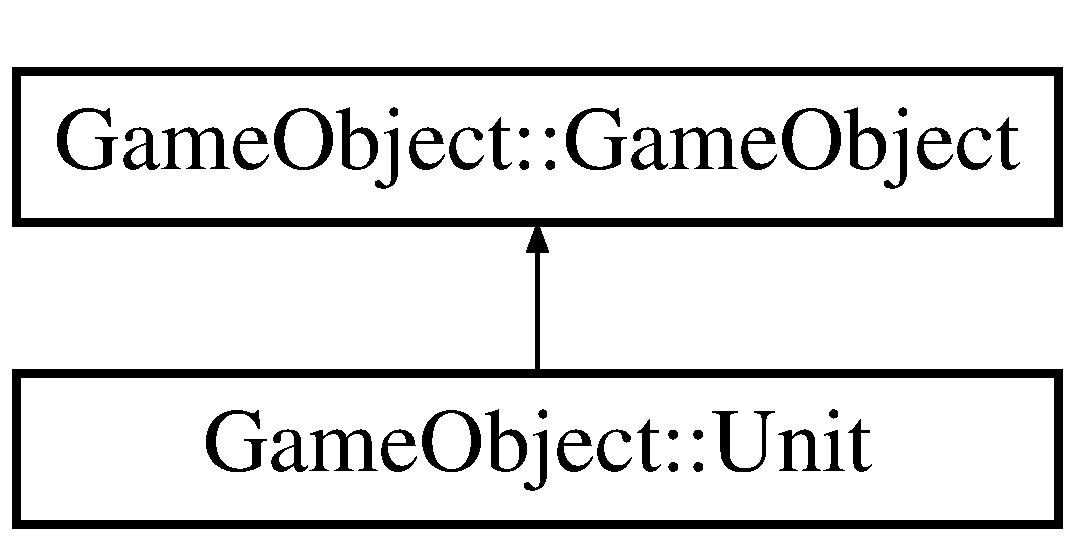
\includegraphics[height=2cm]{classGameObject_1_1Unit}
\end{center}
\end{figure}
\subsection*{Public Member Functions}
\begin{CompactItemize}
\item 
\hypertarget{classGameObject_1_1Unit_29efd7d8ec0ee55b4cfd2a198c42eab5}{
def \textbf{\_\-\_\-init\_\-\_\-}}
\label{classGameObject_1_1Unit_29efd7d8ec0ee55b4cfd2a198c42eab5}

\item 
\hypertarget{classGameObject_1_1Unit_cab27f353a1f56aa6bb1917fd44e59d6}{
def \textbf{validify}}
\label{classGameObject_1_1Unit_cab27f353a1f56aa6bb1917fd44e59d6}

\item 
\hypertarget{classGameObject_1_1Unit_d6ddcef565e5b43deb573300a6cb2b20}{
def \textbf{attack}}
\label{classGameObject_1_1Unit_d6ddcef565e5b43deb573300a6cb2b20}

\item 
\hypertarget{classGameObject_1_1Unit_f067f326af32e3998d449261bc8f23b7}{
def \textbf{build}}
\label{classGameObject_1_1Unit_f067f326af32e3998d449261bc8f23b7}

\item 
\hypertarget{classGameObject_1_1Unit_0875c2b42551b29aaac2964d01196043}{
def \textbf{paint}}
\label{classGameObject_1_1Unit_0875c2b42551b29aaac2964d01196043}

\item 
\hypertarget{classGameObject_1_1Unit_ba05fa00dd08f1344d5ecea04d1633d3}{
def \textbf{move}}
\label{classGameObject_1_1Unit_ba05fa00dd08f1344d5ecea04d1633d3}

\item 
\hypertarget{classGameObject_1_1Unit_e6bb30c8a2f3c1adf9b1c466b712c8ea}{
def \textbf{warp}}
\label{classGameObject_1_1Unit_e6bb30c8a2f3c1adf9b1c466b712c8ea}

\item 
\hypertarget{classGameObject_1_1Unit_14825583af290dbd3303a7655e63a1cd}{
def \textbf{getObjectID}}
\label{classGameObject_1_1Unit_14825583af290dbd3303a7655e63a1cd}

\item 
\hypertarget{classGameObject_1_1Unit_01711efd87c7e3e2a97066e9a5c50da5}{
def \textbf{getX}}
\label{classGameObject_1_1Unit_01711efd87c7e3e2a97066e9a5c50da5}

\item 
\hypertarget{classGameObject_1_1Unit_4d0c47deb0ddb19b9e2b195d8ca2f2ad}{
def \textbf{getY}}
\label{classGameObject_1_1Unit_4d0c47deb0ddb19b9e2b195d8ca2f2ad}

\item 
\hypertarget{classGameObject_1_1Unit_4b32febb0f80ed604833338af2103b16}{
def \textbf{getZ}}
\label{classGameObject_1_1Unit_4b32febb0f80ed604833338af2103b16}

\item 
\hypertarget{classGameObject_1_1Unit_a0e958b475f8e784cab9e443405cc233}{
def \textbf{getHp}}
\label{classGameObject_1_1Unit_a0e958b475f8e784cab9e443405cc233}

\item 
\hypertarget{classGameObject_1_1Unit_b2bf3bbbd066d3b1ec4a6eac3819bb63}{
def \textbf{getLevel}}
\label{classGameObject_1_1Unit_b2bf3bbbd066d3b1ec4a6eac3819bb63}

\item 
\hypertarget{classGameObject_1_1Unit_5dc929b411abd60ea05bc9a45f53ed2c}{
def \textbf{getUnitTypeID}}
\label{classGameObject_1_1Unit_5dc929b411abd60ea05bc9a45f53ed2c}

\item 
\hypertarget{classGameObject_1_1Unit_7a78dc10a8f05d47c6216f0a1cee864e}{
def \textbf{getOwnerID}}
\label{classGameObject_1_1Unit_7a78dc10a8f05d47c6216f0a1cee864e}

\item 
\hypertarget{classGameObject_1_1Unit_d616480400b131d3faad00f63f553c37}{
def \textbf{getActions}}
\label{classGameObject_1_1Unit_d616480400b131d3faad00f63f553c37}

\item 
\hypertarget{classGameObject_1_1Unit_5aa36bd2ed0fa42becc2f3e15c4a2fbb}{
def \textbf{getMoves}}
\label{classGameObject_1_1Unit_5aa36bd2ed0fa42becc2f3e15c4a2fbb}

\end{CompactItemize}
\subsection*{Public Attributes}
\begin{CompactItemize}
\item 
\hypertarget{classGameObject_1_1Unit_eed6c6641d9ab913c271e07ce91f66dc}{
\textbf{ptr}}
\label{classGameObject_1_1Unit_eed6c6641d9ab913c271e07ce91f66dc}

\item 
\hypertarget{classGameObject_1_1Unit_a9e881997b25f4452c57074760815d63}{
\textbf{iteration}}
\label{classGameObject_1_1Unit_a9e881997b25f4452c57074760815d63}

\item 
\hypertarget{classGameObject_1_1Unit_aea5d9c834951a5d317c85b8b4e95f65}{
\textbf{ID}}
\label{classGameObject_1_1Unit_aea5d9c834951a5d317c85b8b4e95f65}

\end{CompactItemize}


\subsection{Detailed Description}


\footnotesize\begin{verbatim}An entitiy that can move around the game and act.
\end{verbatim}
\normalsize
 

The documentation for this class was generated from the following file:\begin{CompactItemize}
\item 
GameObject.py\end{CompactItemize}

\hypertarget{classGameObject_1_1UnitType}{
\section{GameObject::UnitType Class Reference}
\label{classGameObject_1_1UnitType}\index{GameObject::UnitType@{GameObject::UnitType}}
}
Inheritance diagram for GameObject::UnitType::\begin{figure}[H]
\begin{center}
\leavevmode
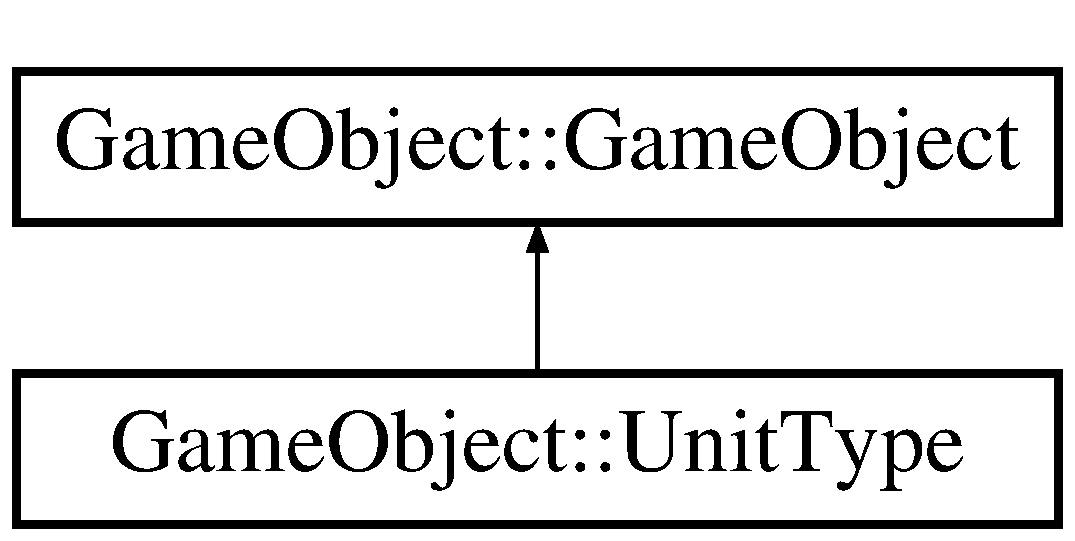
\includegraphics[height=2cm]{classGameObject_1_1UnitType}
\end{center}
\end{figure}
\subsection*{Public Member Functions}
\begin{CompactItemize}
\item 
\hypertarget{classGameObject_1_1UnitType_3888b50f2a13df0000db36e4781cd3ff}{
def \textbf{\_\-\_\-init\_\-\_\-}}
\label{classGameObject_1_1UnitType_3888b50f2a13df0000db36e4781cd3ff}

\item 
\hypertarget{classGameObject_1_1UnitType_9e5978cc4e5b85aa65d62a172a2b651f}{
def \textbf{validify}}
\label{classGameObject_1_1UnitType_9e5978cc4e5b85aa65d62a172a2b651f}

\item 
\hypertarget{classGameObject_1_1UnitType_6f3133c7cb2dccacc082add2f3e6934a}{
def \textbf{getObjectID}}
\label{classGameObject_1_1UnitType_6f3133c7cb2dccacc082add2f3e6934a}

\item 
\hypertarget{classGameObject_1_1UnitType_d0d9d8e7d891016eac956d6221e0603e}{
def \textbf{getName}}
\label{classGameObject_1_1UnitType_d0d9d8e7d891016eac956d6221e0603e}

\item 
\hypertarget{classGameObject_1_1UnitType_8312ce18858f9e073dbf9f4fa89a2fe2}{
def \textbf{getPrice}}
\label{classGameObject_1_1UnitType_8312ce18858f9e073dbf9f4fa89a2fe2}

\item 
\hypertarget{classGameObject_1_1UnitType_3c2b6d72d746dce2ec0d6eb9a5127f2f}{
def \textbf{getHunger}}
\label{classGameObject_1_1UnitType_3c2b6d72d746dce2ec0d6eb9a5127f2f}

\item 
\hypertarget{classGameObject_1_1UnitType_db21e3e80cd8aa24babcf33ae97a8c6d}{
def \textbf{getTrainTime}}
\label{classGameObject_1_1UnitType_db21e3e80cd8aa24babcf33ae97a8c6d}

\item 
\hypertarget{classGameObject_1_1UnitType_b573147e22ec10c1156fea5aa185d201}{
def \textbf{getHp}}
\label{classGameObject_1_1UnitType_b573147e22ec10c1156fea5aa185d201}

\item 
\hypertarget{classGameObject_1_1UnitType_67c32d0040831757af276b4ceab53f4e}{
def \textbf{getArmor}}
\label{classGameObject_1_1UnitType_67c32d0040831757af276b4ceab53f4e}

\item 
\hypertarget{classGameObject_1_1UnitType_f24e195b3c99a698e3b96abf4ece1897}{
def \textbf{getMoves}}
\label{classGameObject_1_1UnitType_f24e195b3c99a698e3b96abf4ece1897}

\item 
\hypertarget{classGameObject_1_1UnitType_f6058b07c8d7dc188eec16c1d4c780f5}{
def \textbf{getActions}}
\label{classGameObject_1_1UnitType_f6058b07c8d7dc188eec16c1d4c780f5}

\item 
\hypertarget{classGameObject_1_1UnitType_3c1137703c52c683b78434b774fc278b}{
def \textbf{getAttackCost}}
\label{classGameObject_1_1UnitType_3c1137703c52c683b78434b774fc278b}

\item 
\hypertarget{classGameObject_1_1UnitType_7407a171f57c203956add546375bf97c}{
def \textbf{getDamage}}
\label{classGameObject_1_1UnitType_7407a171f57c203956add546375bf97c}

\item 
\hypertarget{classGameObject_1_1UnitType_b42245c51dbf03b96f2235de3ecb3bbe}{
def \textbf{getMinRange}}
\label{classGameObject_1_1UnitType_b42245c51dbf03b96f2235de3ecb3bbe}

\item 
\hypertarget{classGameObject_1_1UnitType_d0ee2ff254fb10ef9226b7918f6d5704}{
def \textbf{getMaxRange}}
\label{classGameObject_1_1UnitType_d0ee2ff254fb10ef9226b7918f6d5704}

\item 
\hypertarget{classGameObject_1_1UnitType_570e0b5afa2a6a62d342f5ef79e3299d}{
def \textbf{getTrainerID}}
\label{classGameObject_1_1UnitType_570e0b5afa2a6a62d342f5ef79e3299d}

\item 
\hypertarget{classGameObject_1_1UnitType_cf2b101e7b25c37605d042a28fc92e90}{
def \textbf{getCanPaint}}
\label{classGameObject_1_1UnitType_cf2b101e7b25c37605d042a28fc92e90}

\item 
\hypertarget{classGameObject_1_1UnitType_2ece581579b741c8c418a55fd0a22f7e}{
def \textbf{getArmorExp}}
\label{classGameObject_1_1UnitType_2ece581579b741c8c418a55fd0a22f7e}

\item 
\hypertarget{classGameObject_1_1UnitType_fbd694bc1c9fa4ae43fa4b4d7c73da7c}{
def \textbf{getHpExp}}
\label{classGameObject_1_1UnitType_fbd694bc1c9fa4ae43fa4b4d7c73da7c}

\item 
\hypertarget{classGameObject_1_1UnitType_bcb8ef43e9e461d7c45986fa6eefb080}{
def \textbf{getPriceExp}}
\label{classGameObject_1_1UnitType_bcb8ef43e9e461d7c45986fa6eefb080}

\item 
\hypertarget{classGameObject_1_1UnitType_c549c835fd4e907b84ff2303705a46e6}{
def \textbf{getDamageExp}}
\label{classGameObject_1_1UnitType_c549c835fd4e907b84ff2303705a46e6}

\item 
\hypertarget{classGameObject_1_1UnitType_c41e7e7e52dc8727adbc516d80436961}{
def \textbf{getPaintBase}}
\label{classGameObject_1_1UnitType_c41e7e7e52dc8727adbc516d80436961}

\item 
\hypertarget{classGameObject_1_1UnitType_79a963c9e82fa8b2adea377e5d2db743}{
def \textbf{getPaintLinear}}
\label{classGameObject_1_1UnitType_79a963c9e82fa8b2adea377e5d2db743}

\end{CompactItemize}
\subsection*{Public Attributes}
\begin{CompactItemize}
\item 
\hypertarget{classGameObject_1_1UnitType_02c8aeecd19a6f22db3bcbf76ae57b42}{
\textbf{ptr}}
\label{classGameObject_1_1UnitType_02c8aeecd19a6f22db3bcbf76ae57b42}

\item 
\hypertarget{classGameObject_1_1UnitType_b40da5ccdb5930c478ac8a20ff6309ee}{
\textbf{iteration}}
\label{classGameObject_1_1UnitType_b40da5ccdb5930c478ac8a20ff6309ee}

\item 
\hypertarget{classGameObject_1_1UnitType_8dc3cbd5a4de477054d7357678e37ef8}{
\textbf{ID}}
\label{classGameObject_1_1UnitType_8dc3cbd5a4de477054d7357678e37ef8}

\end{CompactItemize}


\subsection{Detailed Description}


\footnotesize\begin{verbatim}This defines the attributes of a kind of unit.
\end{verbatim}
\normalsize
 

The documentation for this class was generated from the following file:\begin{CompactItemize}
\item 
GameObject.py\end{CompactItemize}

\printindex
\end{document}
